\documentclass{beamer}

\usepackage{pdfpages}
\usepackage{wrapfig}
\usepackage{subfig}
%\usetheme{boxes}
%\usepackage[export]{adjustbox}
%\usepackage{picture}

\title{Predictive Policing \\ \bigskip Marked Spatio-Temporal Point Processes \\ for preventing crime}

% A subtitle is optional and this may be deleted
% \subtitle{Literature review}

\author{Santhosh Narayanan}
% - Give the names in the same order as the appear in the paper.
% - Use the \inst{?} command only if the authors have different
%   affiliation.
\institute{}

\institute[PredPoint] % (optional, but mostly needed)
{ 
  PredPoint Analytics
}

\date{December 2022}

\subject{Applied Statistics}
% This is only inserted into the PDF information catalog. Can be left
% out. 

% If you have a file called "university-logo-filename.xxx", where xxx
% is a graphic format that can be processed by latex or pdflatex,
% resp., then you can add a logo as follows:

% \pgfdeclareimage[height=0.5cm]{university-logo}{university-logo-filename}
% \logo{\pgfuseimage{university-logo}}

% Delete this, if you do not want the table of contents to pop up at
% the beginning of each subsection:

% Let's get started
\begin{document}

\begin{frame}
  \titlepage
\end{frame}

%\begin{frame}{Outline}
% \tableofcontents
  % You might wish to add the option [pausesections]
%\end{frame}

% Section and subsections will appear in the presentation overview
% and table of contents.

{
\setbeamercolor{background canvas}{bg=}
\includepdf[pages=2]{SecondPresentation.pdf}
}

\begin{frame}{Predictive policing}
\begin{itemize}
    \item Repeat victimisation theory suggests that crimes, like earthquakes 
    exhibit clustering in both time and space\bigskip
    \item Model provides probabilistic predictions for the occurrence of 
    specific crime type over any region and time horizon\bigskip
    \item Generate prediction maps that identify hot-spots where the 
    probability of a particular type of crime is high \bigskip
    \item The estimated event genealogy allows investigators to connect a new 
    crime with previous events 
\end{itemize}  
\end{frame}

\begin{frame}{Dataset}
\begin{figure}
    \hspace*{-25px}
    \centering
    \subfloat{{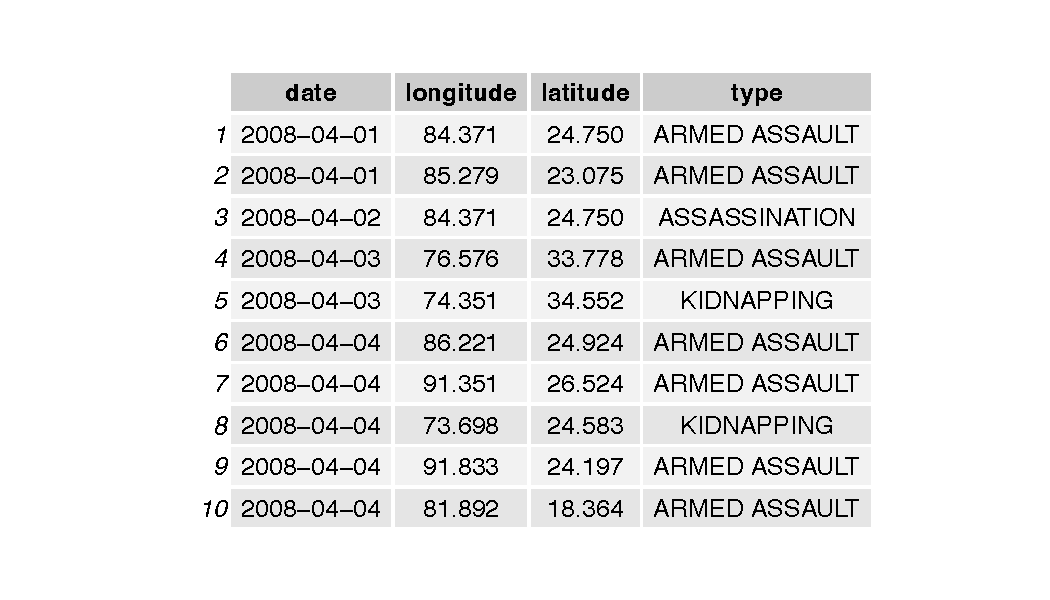
\includegraphics[width = 0.65\linewidth]{figures/DataSnap.pdf} }}
    \subfloat{{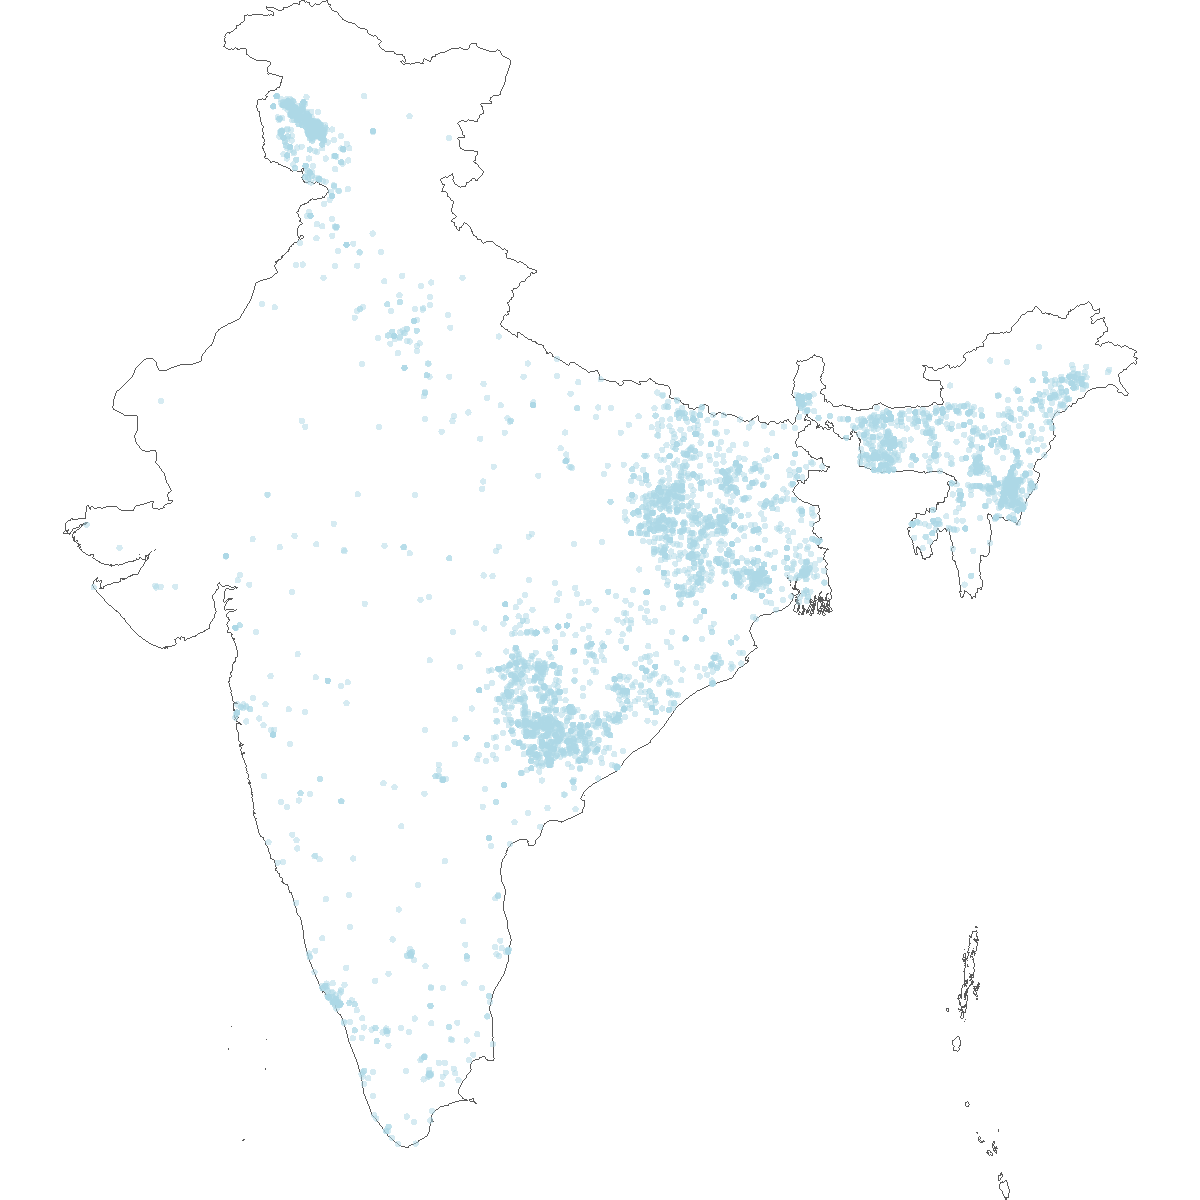
\includegraphics[width = 0.45\linewidth]{figures/DataMap.pdf} }}
\end{figure}
{\footnotesize Source: National Consortium for the Study of Terrorism and Responses to Terrorism (START), University of Maryland. (2019). The Global Terrorism Database (GTD). Retrieved from \url{https://www.start.umd.edu/gtd} }
\end{frame}

\begin{frame}{Observation Region}
\begin{figure}
    \centering
    \subfloat{{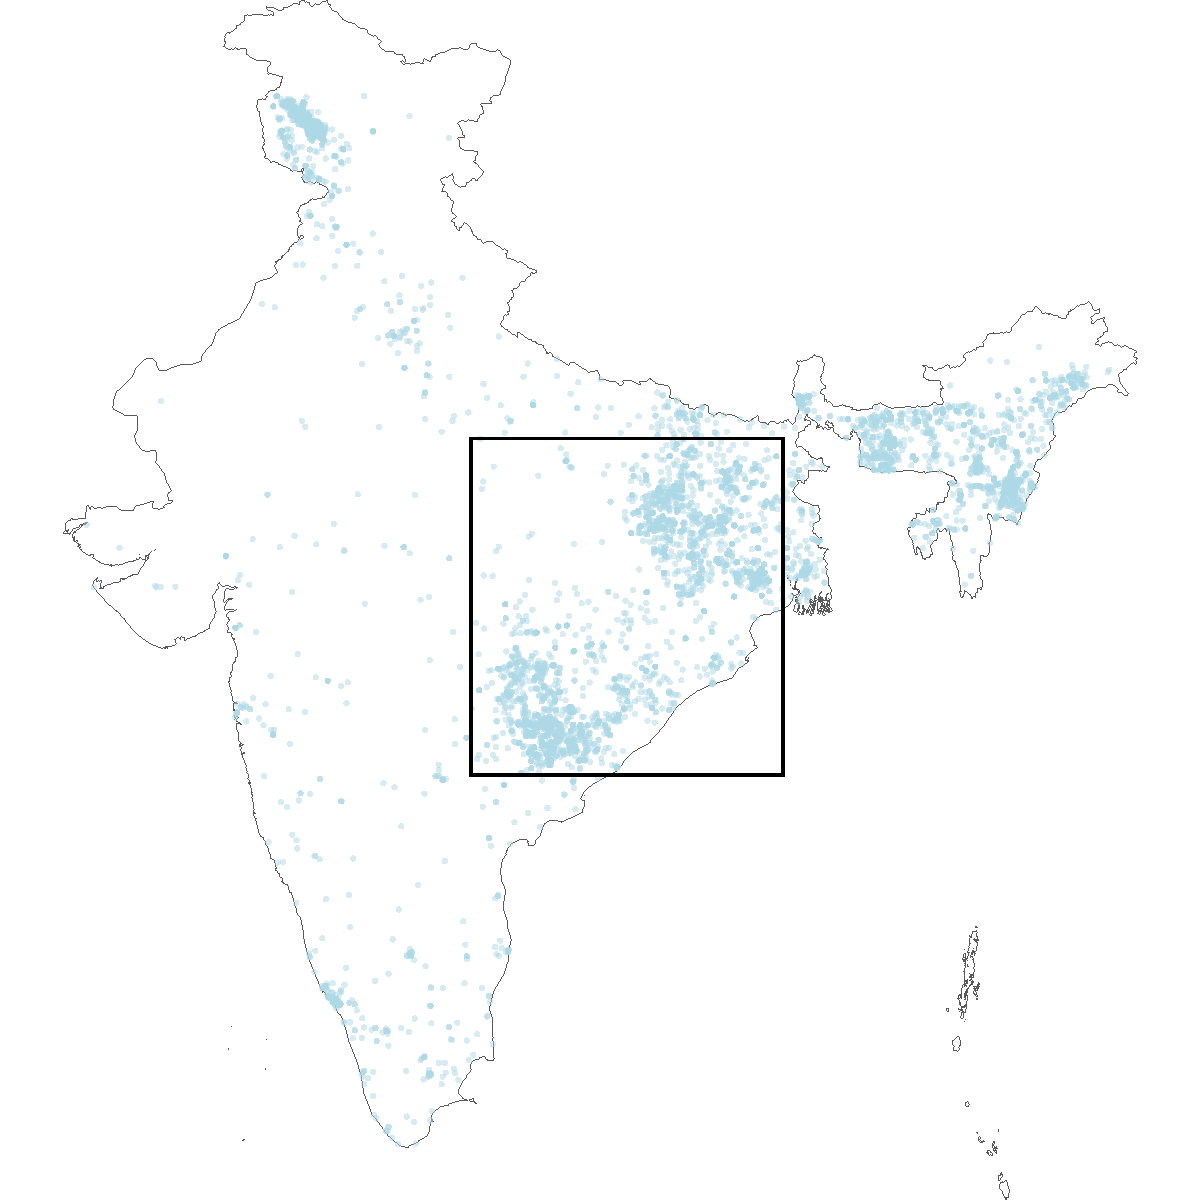
\includegraphics[width = 0.5\linewidth]{figures/FilterMap.pdf} }}
    \subfloat{{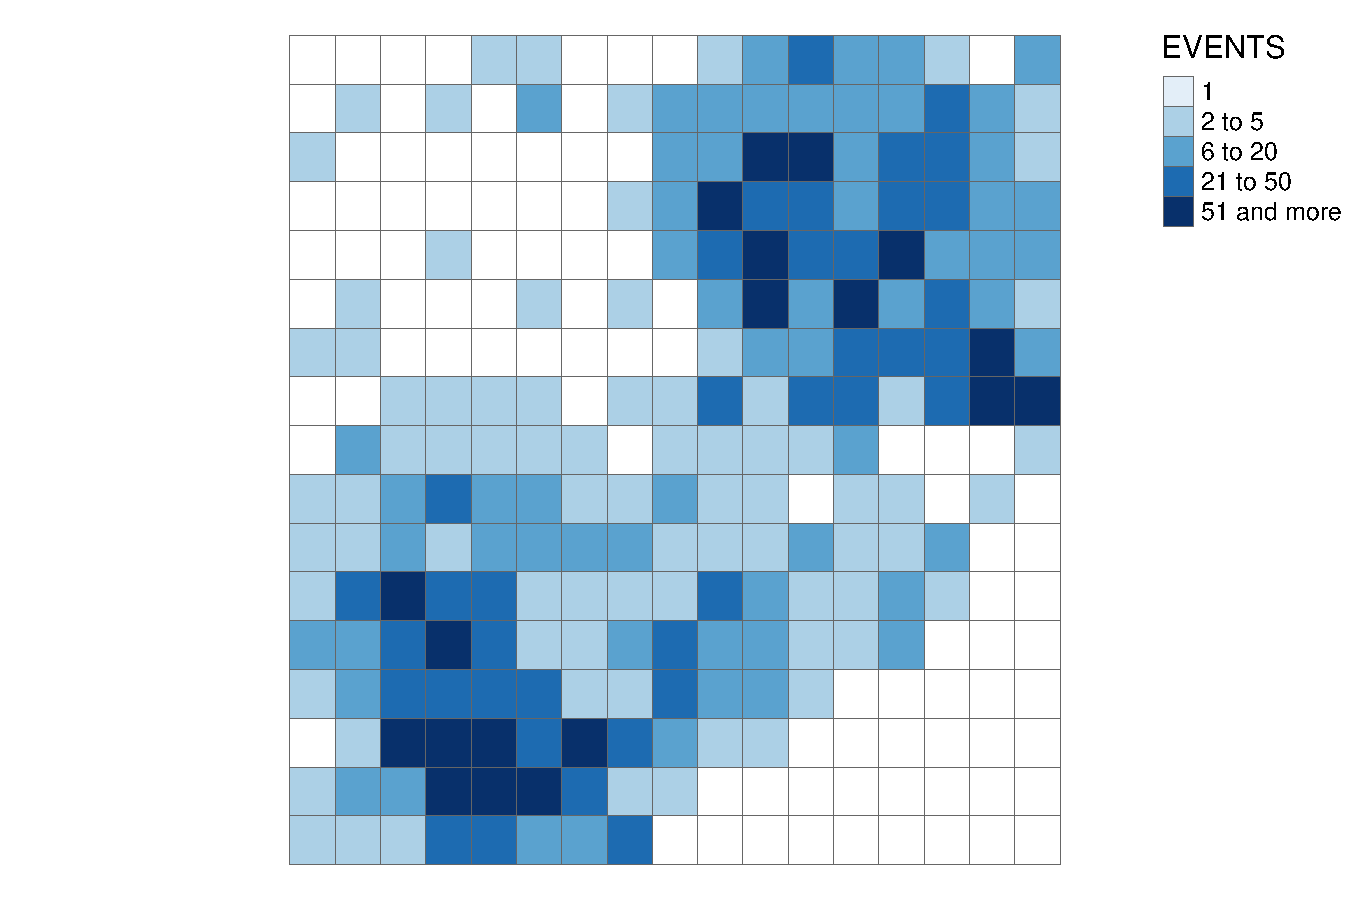
\includegraphics[width = 0.5\linewidth]{figures/GridMapCounts.pdf} }}
\end{figure}
Observation region for experiment and event counts between 1/4/08 and 31/12/19
\end{frame}

\begin{frame}{Second-order analysis}
\begin{figure}
\centering
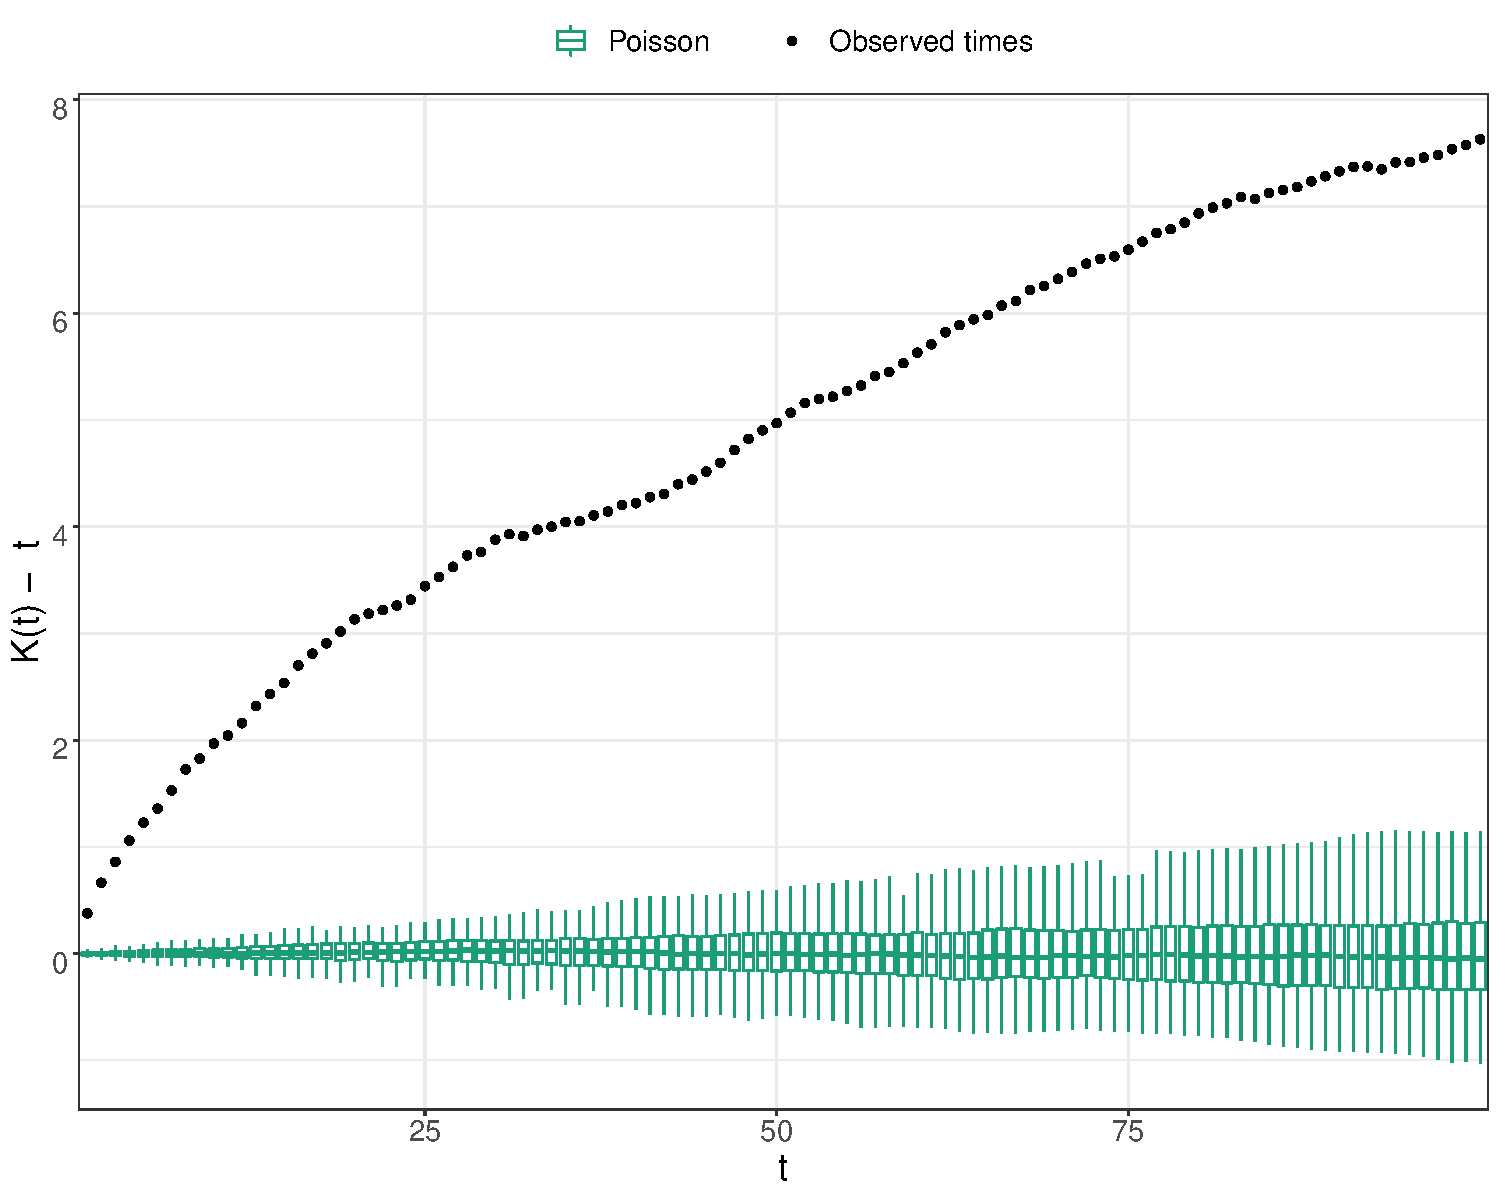
\includegraphics[width = 0.6\linewidth]{figures/Kfuncs.pdf}
\end{figure}
\begin{itemize}
\item The K function is an estimate of the surplus number of events compared to random occurrences
\item The surplus is significant, confirming events cluster in time
\end{itemize}
\end{frame}

\begin{frame}{Prediction Framework}
\begin{itemize}
    \item Generate $S$ simulations of the process in the interval $(T, T + d)$\bigskip
    \item Given the history upto $T$, iteratively simulate the next event, its occurrence time, $(x, y)$ and event type\bigskip
    \item Add the simulated event to the history as the most recent event\bigskip
    \item Stop simulation when the time exceeds $T + d$\bigskip
    \item Finally, aggregate event counts from the $S$ simulations and validate against the observed counts
\end{itemize}   
\end{frame}

\begin{frame}{Validation}
\begin{figure}
    \centering
    \subfloat{{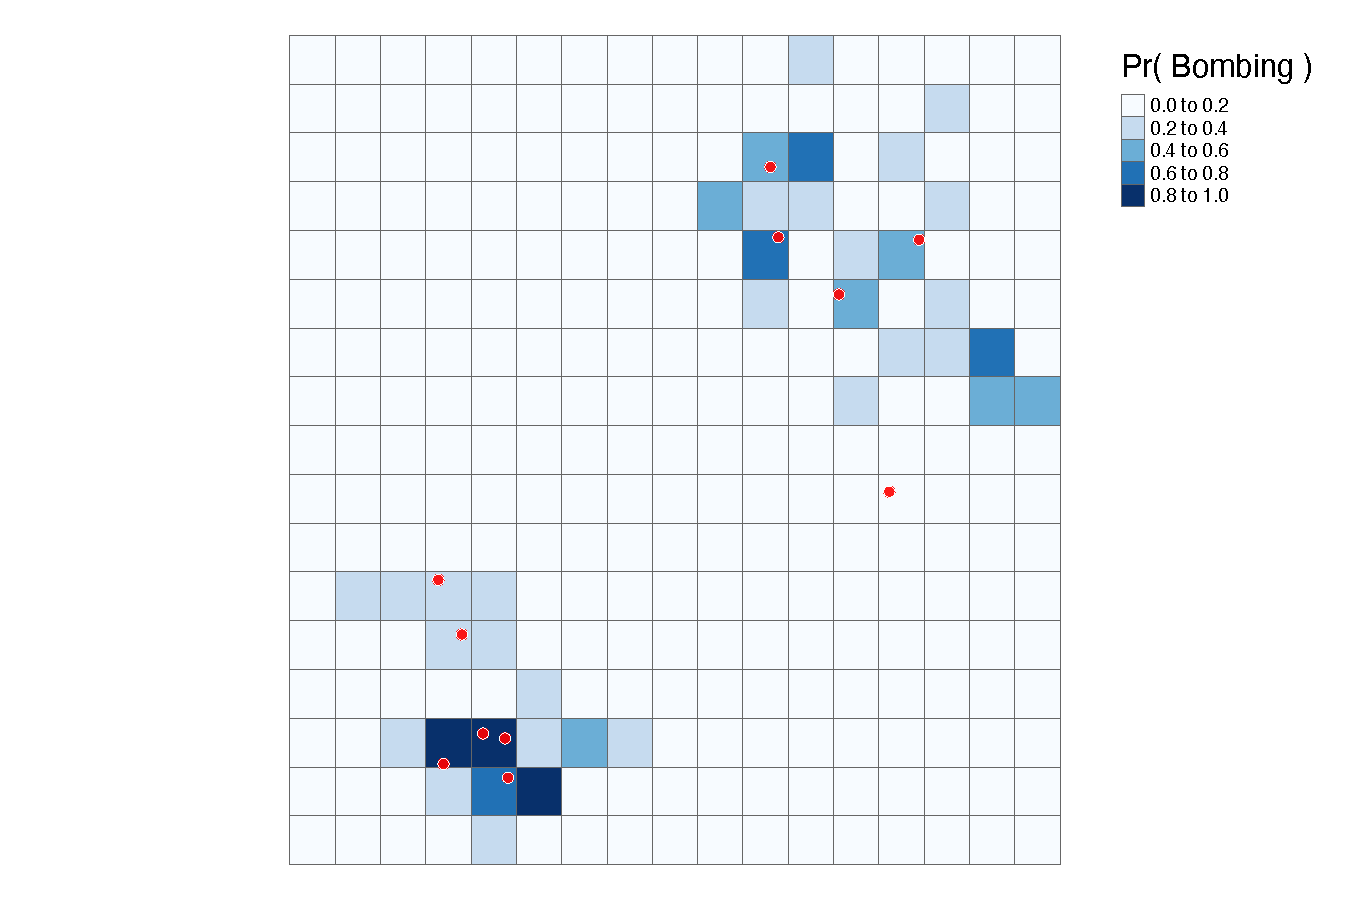
\includegraphics[width = 0.55\linewidth]{figures/Validation.pdf} }}
    \subfloat{{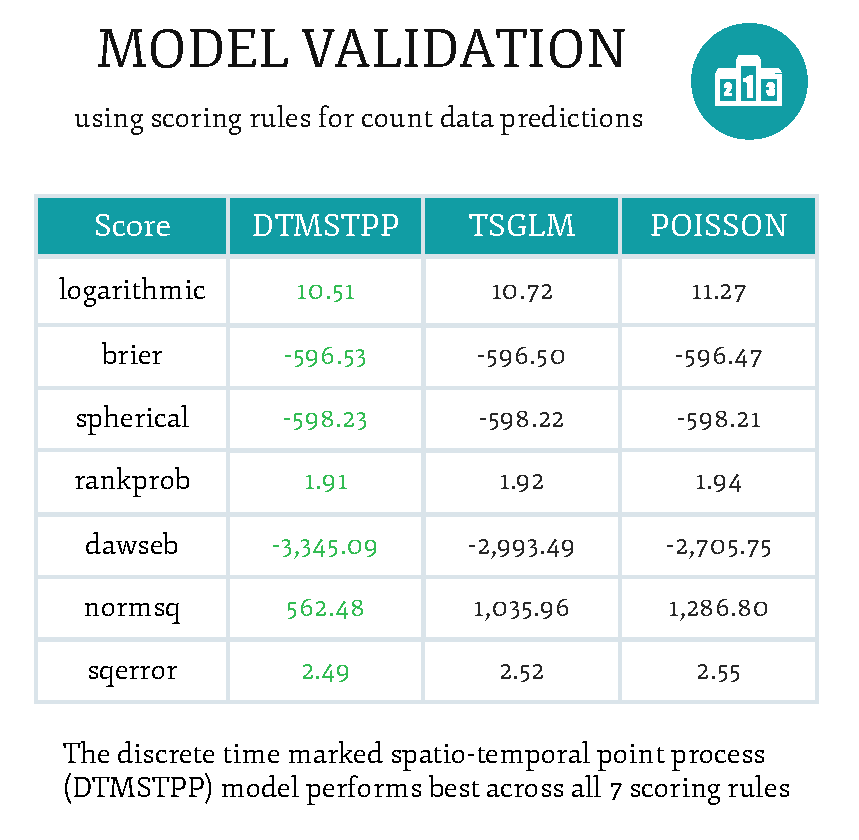
\includegraphics[width = 0.45\linewidth]{figures/Scoring.pdf} }}
\end{figure}
(Left) Prediction Map for the first week in 2018 between 1/1/18 and 7/1/18, based on history up to 31/12/17.
\end{frame}

\begin{frame}{Event Genealogy}
\begin{figure}
\centering
\includegraphics[width = 0.9\linewidth]{figures/Tree.pdf}
\end{figure}
Investigating crimes using the triggering structure.
\end{frame}

\begin{frame}{Learning dynamics}
\begin{figure}
\centering
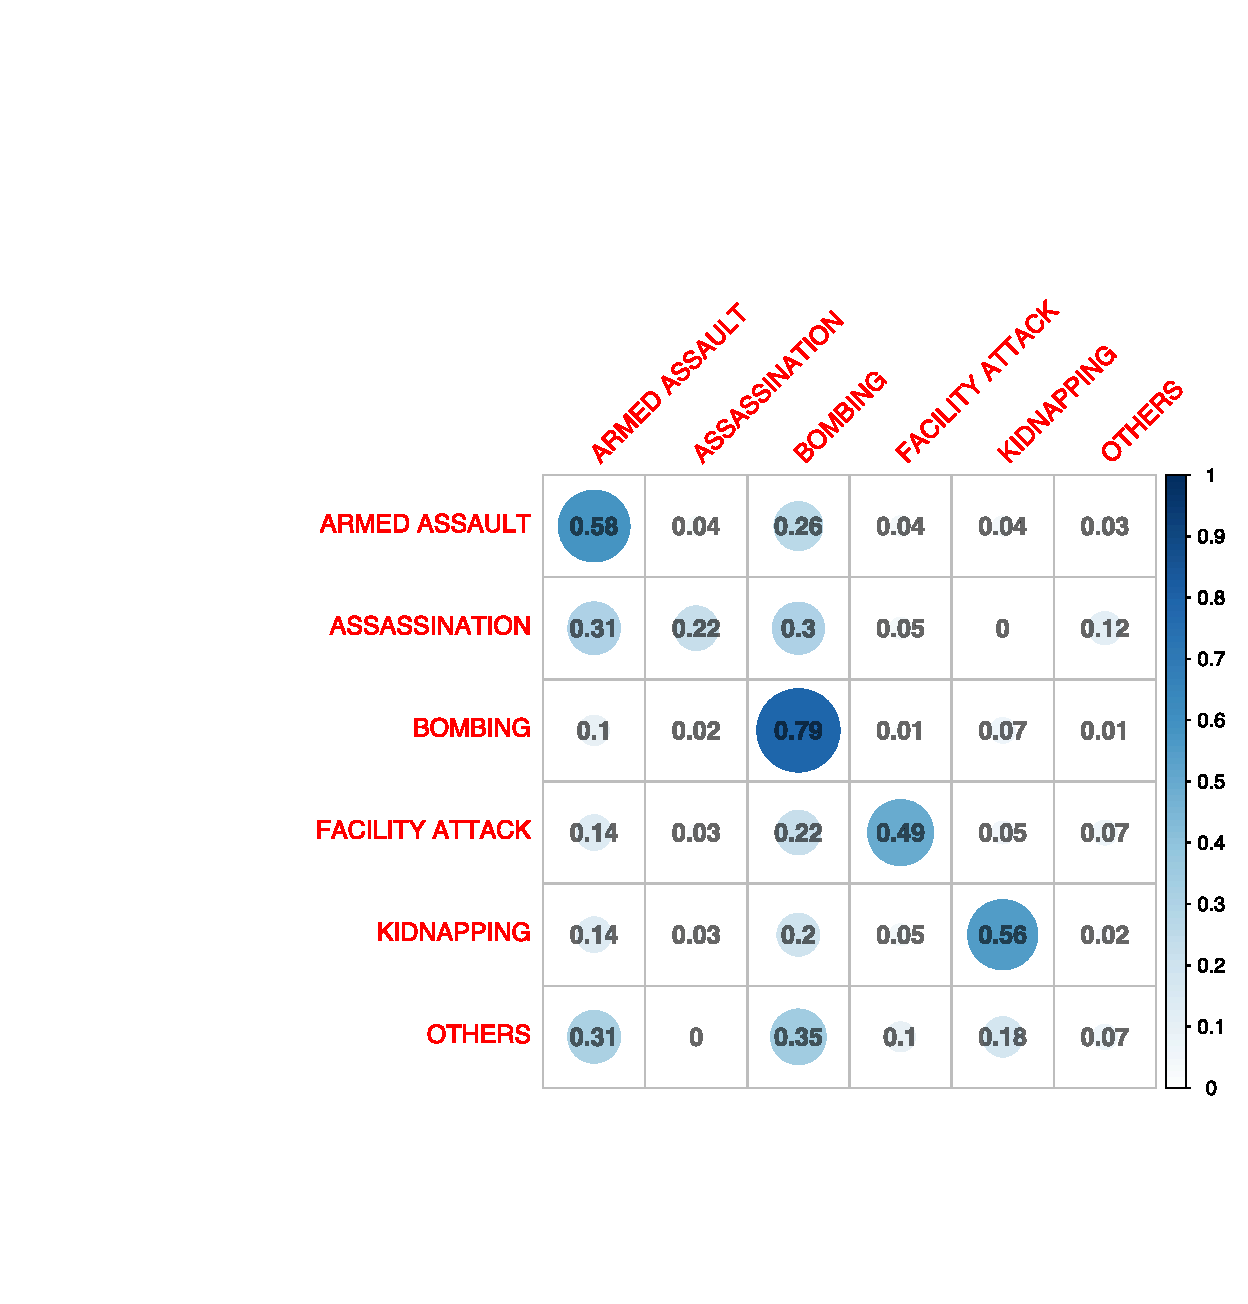
\includegraphics[width = 0.7\linewidth]{figures/CorrPlot.pdf}
\end{figure}
Cross-excitation matrix giving the triggering probabilities between event types.
\end{frame}

{
\setbeamercolor{background canvas}{bg=}
\includepdf[pages=3, scale = 1.2]{SecondPresentation.pdf}
}

{
\setbeamercolor{background canvas}{bg=}
\includepdf[pages=4, scale = 1.2]{SecondPresentation.pdf}
}

{
\setbeamercolor{background canvas}{bg=}
\includepdf[pages=5, scale = 1.4]{SecondPresentation.pdf}
}

\end{document}
